%% =====================================================================
%% paper_additions.tex -- new figures and tables for paper_concise_v8_2
%% Every number below was checked against results/full_v3_20261008/ and
%% results/full_base_20261008/ on branch exp/full-run-v1 (commit 4163ed8),
%% EXCEPT the Selection-Matched Text RAG (SOP-Oracle) values: no oracle
%% system or oracle result exists anywhere in the repository. Those values
%% are copied from the paper text and wrapped in \ifshoworacle ... \fi.
%% Set \showoraclefalse to hide them until the oracle run is committed.
%% =====================================================================

%% ---------------------------------------------------------------------
%% (0) PREAMBLE: add these lines after \usetikzlibrary{...} in the paper
%% ---------------------------------------------------------------------
% \usepackage{pgfplots}
% \pgfplotsset{compat=1.18}
% \newif\ifshoworacle
% \showoracletrue   % <- set to \showoraclefalse to hide unverified oracle values

%% =====================================================================
%% (1) Section 3.2, after the itemize of E1--E3: error class -> metric map
%% =====================================================================
\begin{table}[!htbp]
\centering
\caption{Procedural error classes, the metric used to measure each, and the component of Workflow GraphRAG designed to address it.}
\label{tab:errormap}
\small
\setlength{\tabcolsep}{4pt}
\begin{tabularx}{\textwidth}{>{\raggedright\arraybackslash}p{2.6cm} >{\raggedright\arraybackslash}X >{\raggedright\arraybackslash}p{3.6cm} >{\raggedright\arraybackslash}p{3.0cm}}
\toprule
Error class & Measured by & Design component & Reported in \\
\midrule
E1 Step order inversion & TIR over detected step pairs (Eq.~2); step coverage & \texttt{NEXT\_STEP} traversal and ordered serialization & Table~\ref{tab:results} \\
E2 Actor mismatch & AMR over detected steps with a named actor (Eq.~3) & Per-step actor attribute via \texttt{PERFORMS} & Table~\ref{tab:results}; Section~\ref{sec:audit} \\
E3 Procedural cross-contamination & KFR on cross-SOP and single-SOP questions & Rule-based SOP selection (Eq.~\eqref{eq:score}) & Tables~\ref{tab:percat}, \ref{tab:selection} \\
\bottomrule
\end{tabularx}
\end{table}

%% =====================================================================
%% (2) Section 4.6, after the ablation paragraph: what each system puts
%%     in the prompt. Mean prompt tokens: summary.csv (prompt_tokens_mean).
%% =====================================================================
\begin{figure}[!htbp]
\centering
\resizebox{\textwidth}{!}{%
\begin{tikzpicture}[
  lab/.style={anchor=east, font=\scriptsize, align=right, text width=30mm},
  blk/.style={draw, rounded corners=1.5pt, font=\tiny, align=center, minimum height=6.5mm, minimum width=11mm, inner sep=1pt, fill=white},
  q/.style={blk, minimum width=6mm, fill=gray!15},
  sel/.style={blk, draw=blue!70!black, fill=blue!6, thick, minimum width=23mm},
  trip/.style={blk, fill=gray!30, minimum width=11mm},
  tok/.style={anchor=west, font=\scriptsize}
]
\def\dx{1.2}
% header
\node[font=\scriptsize\bfseries, anchor=east] at (-0.15,0.65) {System};
\node[font=\scriptsize\bfseries, anchor=west] at (0,0.65) {Context passed to the generator (in prompt order)};
\node[font=\scriptsize\bfseries, anchor=west] at (10.2,0.65) {Mean prompt tokens};
% LLM only
\node[lab] at (-0.15,0) {LLM only};
\node[q] at (0.3,0) {$q$};
\node[font=\tiny, anchor=west, text=gray!70!black] at (0.75,0) {no retrieved context};
\node[tok] at (10.2,0) {107};
% Naive
\node[lab] at (-0.15,-0.9) {Naive RAG};
\node[q] at (0.3,-0.9) {$q$};
\foreach \i in {1,2,3} \node[blk] at (0.75+\i*\dx-0.6,-0.9) {chunk\,=\\SOP};
\node[tok] at (10.2,-0.9) {916};
% Entity graph
\node[lab] at (-0.15,-1.8) {GraphRAG (entity)};
\node[q] at (0.3,-1.8) {$q$};
\node[trip] at (1.35,-1.8) {1-hop\\triples};
\foreach \i in {1,2,3} \node[blk] at (1.95+\i*\dx-0.6,-1.8) {chunk\,=\\SOP};
\node[tok] at (10.2,-1.8) {949};
% Workflow
\node[lab] at (-0.15,-2.7) {\textbf{Workflow GraphRAG}};
\node[q] at (0.3,-2.7) {$q$};
\node[sel] at (1.95,-2.7) {workflow block\\of selected $p^\ast$};
\foreach \i in {1,2,3} \node[blk] at (3.15+\i*\dx-0.6,-2.7) {chunk\,=\\SOP};
\node[tok] at (10.2,-2.7) {1,525};
% Selection-matched
\ifshoworacle
\node[lab] at (-0.15,-3.6) {Selection-Matched Text (ablation)};
\node[q] at (0.3,-3.6) {$q$};
\node[sel, thin, fill=blue!3] at (1.95,-3.6) {raw PDF text\\of selected $p^\ast$};
\foreach \i in {1,2,3} \node[blk] at (3.15+\i*\dx-0.6,-3.6) {chunk\,=\\SOP};
\node[tok] at (10.2,-3.6) {1,479};
\fi
% Full context
\node[lab] at (-0.15,-4.5) {Full context};
\node[q] at (0.3,-4.5) {$q$};
\foreach \i in {1,...,7} \node[blk] at (0.75+\i*\dx-0.6,-4.5) {SOP \i};
\node[tok] at (10.2,-4.5) {2,722};
\end{tikzpicture}}
\caption{Context supplied to the generator by the main comparison systems. Because every SOP fits in one 1,700-character chunk, each retrieved chunk is a complete SOP, so top-3 retrieval always places three procedures in the prompt (Section~3.3). Workflow GraphRAG and the selection-matched ablation share the selection rule and the same top-3 supporting chunks, which may come from unselected SOPs, and differ only in how the selected procedure $p^\ast$ is represented. Token counts are means over all 40 questions and include the shared prompt template and question.}
\label{fig:prompt}
\end{figure}

%% =====================================================================
%% (3) Section 6.1 or 6.2, after Table 7 or after the Wilcoxon paragraph:
%%     forest plot of paired KFR differences (significance.csv).
%% =====================================================================
\begin{figure}[!htbp]
\centering
\begin{tikzpicture}
\begin{axis}[
  width=0.78\textwidth, height=5.0cm,
  xmin=-0.12, xmax=0.47, ymin=0.4, ymax=4.6,
  ytick={1,2,3,4},
  yticklabels={
    \ifshoworacle Workflow $-$ Selection-Matched\else\fi,
    Full context $-$ Naive RAG,
    Workflow $-$ GraphRAG (entity),
    Workflow $-$ Naive RAG},
  yticklabel style={font=\scriptsize, align=right},
  xticklabel style={font=\scriptsize, /pgf/number format/fixed, /pgf/number format/precision=2},
  xlabel={Paired mean difference in key-fact recall ($n=35$), 95\% bootstrap CI},
  xlabel style={font=\scriptsize},
  axis lines*=left, tick align=outside, clip=false,
  xmajorgrids, grid style={gray!20},
]
\draw[gray!70, dashed] (axis cs:0,0.4) -- (axis cs:0,4.6);
% Workflow - Naive: 0.243 [0.114, 0.381], Holm p = 0.053
\addplot[blue!70!black, only marks, mark=square*, mark size=2.2pt, error bars/.cd, x dir=both, x explicit, error bar style={thick}]
  coordinates {(0.243,4) += (0.138,0) -= (0.129,0)};
% Workflow - GraphRAG: 0.257 [0.133, 0.395], Holm p = 0.034
\addplot[blue!70!black, only marks, mark=square*, mark size=2.2pt, error bars/.cd, x dir=both, x explicit, error bar style={thick}]
  coordinates {(0.257,3) += (0.138,0) -= (0.124,0)};
% Full context - Naive: 0.250 [0.121, 0.400], Holm p = 0.053
\addplot[black, only marks, mark=triangle*, mark size=2.4pt, error bars/.cd, x dir=both, x explicit, error bar style={thick}]
  coordinates {(0.250,2) += (0.150,0) -= (0.129,0)};
\ifshoworacle
% Workflow - Selection-Matched: -0.007 [-0.036, 0.021], Wilcoxon p = 0.59 (paper text; not in repository)
\addplot[blue!70!black, only marks, mark=square, mark size=2.2pt, error bars/.cd, x dir=both, x explicit, error bar style={thick}]
  coordinates {(-0.007,1) += (0.028,0) -= (0.029,0)};
\node[font=\scriptsize, anchor=west] at (axis cs:0.405,1) {$p=0.59$};
\fi
\node[font=\scriptsize, anchor=west] at (axis cs:0.405,4) {$p_{\mathrm{Holm}}=0.053$};
\node[font=\scriptsize, anchor=west] at (axis cs:0.405,3) {$p_{\mathrm{Holm}}=0.034$};
\node[font=\scriptsize, anchor=west] at (axis cs:0.405,2) {$p_{\mathrm{Holm}}=0.053$};
\end{axis}
\end{tikzpicture}
\caption{Paired differences in key-fact recall on the 35 answerable questions, with 95\% bootstrap confidence intervals and two-sided Wilcoxon signed-rank $p$-values (Holm-adjusted within each reference family). Gains over chunk retrieval appear for both Workflow GraphRAG and full-context prompting, whereas the selection-matched comparison, which holds procedure selection fixed, is centred near zero.}
\label{fig:forest}
\end{figure}

%% =====================================================================
%% (4) Section 6.4, after Table 8: recall versus prompt tokens.
%%     KFR and CI: summary.csv; prompt tokens: prompt_tokens_mean.
%% =====================================================================
\begin{figure}[!htbp]
\centering
\begin{tikzpicture}
\begin{axis}[
  width=0.82\textwidth, height=6.4cm,
  xmin=0, xmax=3000, ymin=0, ymax=1.05,
  xlabel={Mean prompt tokens per question (all 40 questions)},
  ylabel={Key-fact recall ($n=35$)},
  xlabel style={font=\scriptsize}, ylabel style={font=\scriptsize},
  ticklabel style={font=\scriptsize},
  scaled x ticks=false, xtick={0,500,...,3000}, xticklabel style={/pgf/number format/1000 sep={}},
  axis lines*=left, tick align=outside, clip=false,
  grid=major, grid style={gray!20},
  error bars/error bar style={gray!70},
]
% chunk-retrieval baselines
\addplot[black, only marks, mark=*, mark size=1.8pt, error bars/.cd, y dir=both, y explicit]
coordinates {
 (916,0.712)  += (0,0.128) -= (0,0.141)
 (882,0.683)  += (0,0.136) -= (0,0.147)
 (949,0.698)  += (0,0.131) -= (0,0.138)
 (994,0.702)  += (0,0.129) -= (0,0.140)
 (1815,0.712) += (0,0.128) -= (0,0.141)
 (725,0.569)  += (0,0.150) -= (0,0.155)
};
% reference systems
\addplot[black, only marks, mark=triangle*, mark size=2.4pt, error bars/.cd, y dir=both, y explicit]
coordinates {
 (107,0.113)  += (0,0.070) -= (0,0.063)
 (2722,0.962) += (0,0.038) -= (0,0.048)
};
% proposed
\addplot[blue!70!black, only marks, mark=square*, mark size=2.2pt, error bars/.cd, y dir=both, y explicit]
coordinates {(1525,0.955) += (0,0.035) -= (0,0.038)};
\ifshoworacle
\addplot[blue!70!black, only marks, mark=square, mark size=2.2pt, error bars/.cd, y dir=both, y explicit]
coordinates {(1479,0.962) += (0,0.038) -= (0,0.048)};
\node[font=\tiny, anchor=east, blue!70!black] at (axis cs:1440,1.01) {Selection-Matched};
\fi
% labels
\node[font=\tiny, anchor=north west] at (axis cs:1010,0.62) {Naive, Hybrid, GraphRAG, Multimodal};
\draw[gray!70, thin] (axis cs:1000,0.62) -- (axis cs:960,0.67);
\node[font=\tiny, anchor=north] at (axis cs:725,0.40) {CRAG};
\node[font=\tiny, anchor=west] at (axis cs:1850,0.712) {Agentic};
\node[font=\tiny, anchor=west] at (axis cs:150,0.113) {LLM only};
\node[font=\tiny, anchor=north east, blue!70!black] at (axis cs:1500,0.93) {\textbf{Workflow GraphRAG}};
\node[font=\tiny, anchor=east] at (axis cs:2680,0.962) {Full context};
\draw[{Stealth[length=1.6mm]}-{Stealth[length=1.6mm]}, gray!70!black] (axis cs:1545,0.88) -- node[above, font=\tiny]{$-44\%$ prompt tokens} (axis cs:2702,0.88);
\end{axis}
\end{tikzpicture}
\caption{Key-fact recall against mean prompt tokens for all evaluated systems. Error bars show 95\% bootstrap confidence intervals. Circles: chunk-retrieval baselines; triangles: reference systems; squares: systems using rule-based SOP selection. Workflow GraphRAG reaches recall numerically close to full-context prompting with 44\% fewer prompt tokens.}
\label{fig:tradeoff}
\end{figure}

%% =====================================================================
%% (5) Section 6.2, replacing the long selection paragraph (or after it):
%%     selector outcome per item group (generations.jsonl: matched_sop).
%% =====================================================================
\begin{table}[!htbp]
\centering
\caption{Outcome of the rule-based SOP selector (Eq.~\eqref{eq:score}) for Workflow GraphRAG on all 40 benchmark questions, read from the \texttt{matched\_sop} field of the run log.}
\label{tab:selection}
\small
\setlength{\tabcolsep}{4pt}
\begin{tabularx}{\textwidth}{>{\raggedright\arraybackslash}p{3.6cm} r >{\raggedright\arraybackslash}X >{\raggedright\arraybackslash}p{3.4cm}}
\toprule
Question group & $n$ & Selector outcome & Consequence \\
\midrule
Answerable, single SOP & 32 & Correct SOP selected (32/32) & Workflow block of correct SOP in prompt \\
Answerable, cross-SOP (X-1--X-3) & 3 & One of the involved SOPs selected (X-1: Reactivation; X-2: Academic leave; X-3: Course registration) & Other SOPs reach the prompt only via supporting chunks \\
Unanswerable, SOP topic (NA-1--NA-3) & 3 & Topical SOP selected & Generator abstained (3/3) \\
Unanswerable, no match (NA-4, NA-5) & 2 & No SOP reaches $s \geq 3$ & Deterministic refusal before generation \\
\midrule
Total & 40 & No misrouting between procedures & \\
\bottomrule
\end{tabularx}
\end{table}

%% =====================================================================
%% (6) Section 6.5: embedding ablation as a slope chart (can replace Table 9).
%%     v3: full_v3_20261008/summary.csv; base: full_base_20261008/summary.csv
%% =====================================================================
\begin{figure}[!htbp]
\centering
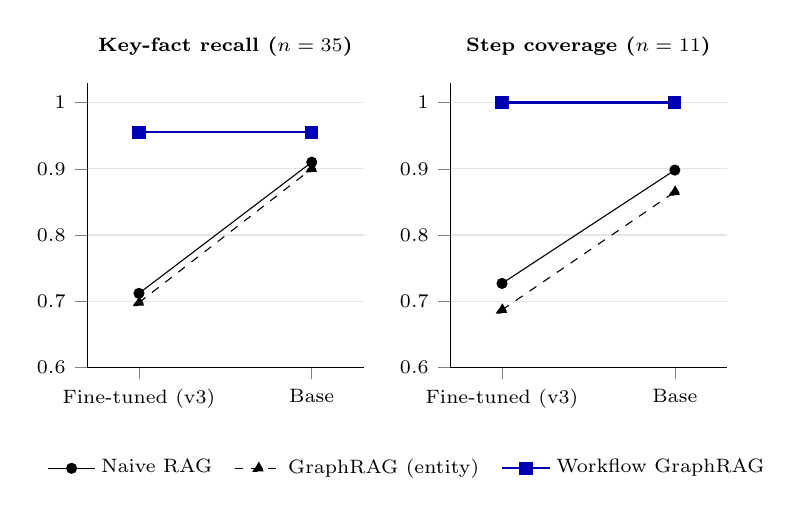
\begin{tikzpicture}
\pgfplotsset{abl/.style={
  width=0.42\textwidth, height=5.2cm,
  xmin=-0.3, xmax=1.3, ymin=0.6, ymax=1.03,
  xtick={0,1}, xticklabels={Fine-tuned (v3), Base},
  ticklabel style={font=\scriptsize}, title style={font=\scriptsize\bfseries},
  axis lines*=left, tick align=outside, ymajorgrids, grid style={gray!20},
  yticklabel style={/pgf/number format/fixed, /pgf/number format/precision=2}}}
\begin{axis}[abl, name=kfr, title={Key-fact recall ($n=35$)}]
\addplot[black, mark=*, mark size=1.8pt] coordinates {(0,0.712) (1,0.910)};
\addplot[black, dashed, mark=triangle*, mark size=2.2pt] coordinates {(0,0.698) (1,0.900)};
\addplot[blue!70!black, thick, mark=square*, mark size=2pt] coordinates {(0,0.955) (1,0.955)};
\end{axis}
\begin{axis}[abl, at={(kfr.east)}, anchor=west, xshift=1.1cm, title={Step coverage ($n=11$)},
  legend style={font=\scriptsize, draw=none, at={(-0.15,-0.28)}, anchor=north, legend columns=3, /tikz/every even column/.append style={column sep=6pt}}]
\addplot[black, mark=*, mark size=1.8pt] coordinates {(0,0.727) (1,0.898)};
\addplot[black, dashed, mark=triangle*, mark size=2.2pt] coordinates {(0,0.687) (1,0.865)};
\addplot[blue!70!black, thick, mark=square*, mark size=2pt] coordinates {(0,1.000) (1,1.000)};
\legend{Naive RAG, GraphRAG (entity), Workflow GraphRAG}
\end{axis}
\end{tikzpicture}
\caption{Embedding sensitivity: key-fact recall and step coverage with the fine-tuned (v3) and the non-fine-tuned base \texttt{all-indo-e5-small-v4} embedding. Chunk-retrieval baselines improve markedly with the base model, whereas Workflow GraphRAG is unchanged.}
\label{fig:embedding}
\end{figure}

%% =====================================================================
%% (7) APPENDIX B: entity-graph baseline triples (src/engine.py, lines 176-192)
%% =====================================================================
% \section{Entity-graph baseline triples}
% \label{app:triples}
\begin{table}[!htbp]
\centering
\caption{The 17 hand-curated relational triples of the custom entity-graph GraphRAG baseline, as defined in \texttt{src/engine.py}. Entities and relations are kept in their original Indonesian form.}
\label{tab:triples}
\scriptsize
\setlength{\tabcolsep}{4pt}
\begin{tabular}{rlll}
\toprule
\# & Head entity & Tail entity & Relation \\
\midrule
1 & cuti akademik & izin cuti & prosedur pengajuan \\
2 & cuti akademik & aktif kembali & alur lanjutan \\
3 & cuti akademik & ketua program studi & rekomendasi \& persetujuan \\
4 & cuti akademik & dekan & penerbitan SK izin \\
5 & cuti akademik & spp/ukt & syarat bebas tunggakan \\
6 & legalisir & ijazah & dokumen objek \\
7 & legalisir & transkrip & dokumen objek \\
8 & legalisir & subbagian akademik & verifikasi \& validasi \\
9 & beasiswa & rekomendasi beasiswa & dokumen pengajuan \\
10 & beasiswa & wakil dekan i & pengesahan surat \\
11 & ukt & keterlambatan pembayaran & permohonan dispensasi \\
12 & ukt & bagian keuangan fsm & verifikasi pembayaran \\
13 & irs & pengisian irs & registrasi akademik per semester \\
14 & irs & dosen wali & bimbingan \& persetujuan online \\
15 & irs & siap undip & portal sistem informasi \\
16 & organisasi mahasiswa & proposal kegiatan & pengajuan persetujuan \\
17 & organisasi mahasiswa & wakil dekan i & persetujuan kegiatan \\
\bottomrule
\end{tabular}
\end{table}

%% =====================================================================
%% (8) APPENDIX C: one benchmark question per category
%%     (benchmark/sop_benchmark_v1.json; English glosses are ours)
%% =====================================================================
% \section{Example benchmark questions}
% \label{app:examples}
\begin{table}[!htbp]
\centering
\caption{One benchmark question per category from \texttt{sop\_benchmark\_v1.json}, with English glosses.}
\label{tab:examples}
\scriptsize
\setlength{\tabcolsep}{3pt}
\begin{tabularx}{\textwidth}{l l >{\raggedright\arraybackslash}X}
\toprule
ID & Category & Question (Indonesian) / English gloss \\
\midrule
CUTI-P1 & Procedural & \textit{Apa saja tahapan mengajukan cuti akademik di FSM dari awal sampai surat izin keluar, dan siapa yang mengerjakan tiap tahap?} \newline What are the steps for applying for academic leave at FSM, from the start until the permit letter is issued, and who performs each step? \\
CUTI-A1 & Actor & \textit{Setelah form cuti saya ditandatangani Kaprodi, form itu diserahkan ke siapa dan diproses oleh bagian apa?} \newline After the Head of Study Programme signs my leave form, to whom is it submitted and which unit processes it? \\
CUTI-D1 & Documents & \textit{Dokumen apa saja yang harus dilampirkan saat mengajukan cuti akademik?} \newline Which documents must be attached when applying for academic leave? \\
CUTI-T1 & Time/location & \textit{Berapa lama maksimal proses izin cuti akademik, dan di mana saya mengambil Surat Izin Dekan?} \newline What is the maximum processing time for an academic leave permit, and where do I collect the Dean's permit letter? \\
X-1 & Cross-SOP & \textit{Apa perbedaan dokumen yang dibawa untuk mengajukan cuti akademik dengan untuk aktif kembali setelah cuti?} \newline How do the documents required for academic leave differ from those required for reactivation after leave? \\
NA-1 & Unanswerable & \textit{Berapa biaya legalisir ijazah per lembar di FSM?} \newline How much does diploma legalisation cost per sheet at FSM? \\
\bottomrule
\end{tabularx}
\end{table}
